\documentclass[a4paper,m]{cgBA}
\usepackage[utf8]{inputenc}
\usepackage[ngerman]{babel}
%\usepackage[T1]{fontenc}

%equations,symbols
\usepackage{amsmath}
\usepackage{amsfonts}
\usepackage{amssymb}
\usepackage{gensymb}
\usepackage{algorithm2e}


%figures
\usepackage{caption}
\usepackage{graphicx}
\usepackage{listings}
\usepackage{color}
\usepackage{subcaption}

\renewcommand{\algorithmcfname}{Algorithmus}
\renewcommand{\lstlistingname}{Quellcode}

\definecolor{mygreen}{rgb}{0,0.6,0}

\lstdefinestyle{customc}{
  breaklines=true,
  %morekeywords{float4,},
  frame=single,
  language=C,
  showstringspaces=false,
  basicstyle=\footnotesize\ttfamily,
  keywordstyle=\bfseries\color{blue},
  commentstyle=\itshape\color{mygreen},
  identifierstyle=\color{black},
  stringstyle=\color{orange},
  tabsize=2,
}


%misc
\usepackage[hidelinks]{hyperref}

\newcommand*{\etal}{\textit{\,et\,al}.~}

\title{Simulation von Haaren und Fell}
\author{Benedikt-Johannes Kraus}
\zweitgutachter{M.\,Sc.\,Kevin Keul}
\zweitgutachterInfo{(Institut für Computervisualistik, AG Computergraphik)}

\begin{document}
\maketitle

\pagenumbering{roman}
\tableofcontents
\clearpage
\pagenumbering{arabic}


\section{Einleitung}

\section{Grundlagen}

\subsection{Sarkomer}

\subsubsection{Myosin}

\subsubsection{Aktin}

\section{Implementation}
Jedes Sarkomer besteht aus Myosin und Aktin Filamenten.
Die in dieser Arbeit betrachteten Sarkomere unterscheiden sich vor allem durch die Anordnung des Aktins. 
Das in dieser Arbeit vorgestellte Programm erlaubt es dem Benutzer am Anfang mit einer Gui eine von vier vorgegeben Sarkomer Strukturen auszuwählen. Außerdem müssen am Anfang Startparameter  angegeben werden um das Modell erzeugen zu können. Diese Parameter sind die Länge der Aktin Filamente (\(lengthActin\)), ein Abstandsmaß zwischen zwei Myosin Filamenten (\(d10\)) welcher sich aus der Dichte des Sarkomers ab leiteten lässt, der Anzahl der Myosin Filamente (\(numMyosin\)) und der Position des Sarkomers (\(posSarcomere\)). Alle weiteren Parameter des Sarkomers sind im Verhältnis zu diesen Grundwerten definiert.

Nachdem alle Grundparameter angegeben wurden kann ein Sarkomer erstellt werden. Im Nachhinein sind über die Gui fast alle Parameter nachträglich anpassbar. Dadurch ist gewährleistet das alle möglichen Formen von Sarkomeren im Rahmen der vier vorgestellten Grundtypen mit dem Programm nachgebaut werden können.  

\subsection{Generierung von Myosin}

\begin{figure}[h]
\center
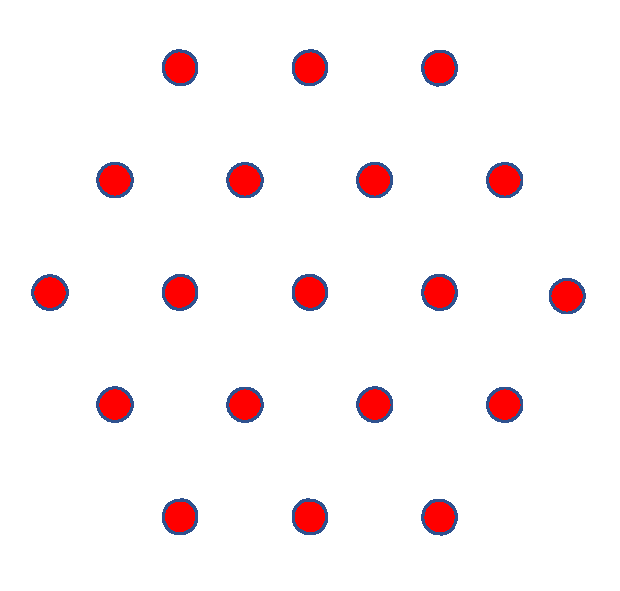
\includegraphics[width=0.5\textwidth]{Graphics/MyosinGitter.pdf}
\caption{MyosinGitter}
\label{fig:MyosinGitter}
\end{figure}

Die Anordnung der Myosinfilamente ist in jedem der vorgestellten Sarkomer Formen gleich. Diese ist wie in (....) beschrieben ein zentriertes Sechseck (siehe Abbildung \ref{fig:MyosinGitter}. Weiterhin hat jedes Myosin Filament die gleiche Geometrie wodurch es sich anbietet, diese nur einmal zu generieren und diese dann mit \textit{Instanced Rendering} im Vertex Shader an \(x\) vorher berechnete Positionen zu verschieben. 

\subsubsection{Generierung der Myosin Offset Positionen}

Die erste Myosin Position wird auf die Position des Sarkomers \(posSarcomere\) gelegt. Dadurch wird festgelegt das \(posSarcomere\) im Mittelpunkt des Sarkomers liegt. Danach werden alle weiteren Myosin Positionen kreisförmig von der Mitte anfangend nach außen angeordnet bis die gewünschte Anzahl an Myosin Positionen befüllt wurde. Dabei füllt das Programm den letzten ``Kreis'' auf, auch wenn dadurch die vom Benutzer angegebene Anzahl von Myosin Filamenten \(numMyosin\) überschritten wird. Dadurch ergibt sich am Ende ein Wohlgeformtes Sechseckiges Sarkomer mit einer Anzahl an Myosin Filamenten die die Form \(3n^2 -3n +1\) (zentrierte Sechseckzahl) aufweist. 

Nachdem die Mittlere Position gesetzt wurde, werden pro Schleifendurchlauf sechs Stützpositionen im Kreis um den Mittelpunkt angeordnet. Dazu wird die Mittlere Position um \(dMyosin * cycleCount = \frac{2 * d10}{\sqrt{3}} * cycleCount\), den Abstand zwischen zwei Myosin Filamenten in Abhängigkeit von \(d10\) multipliziert mit dem aktuellen Schleifendurchlauf \(cycleCount\) in x-Richtung verschoben und dann um \(0, 60, 120...\) Grad rotiert bis der Kreis bzw. das Sechseck geschlossen ist.	

Anschließend werden ab dem zweiten Schleifendurchlauf auf der Strecke zwischen jeder benachbarten Stützposition weitere Zwischenpositionen erzeugt.
Die Anzahl der zwischen jeweils zwei Stützpositionen neu zu erzeugenden Zwischenposition ist \(n = cycleCount - 1\). Um die neuen Positionen zu berechnen wird also die Strecke zwischen jeweils zwei Stützpositionen in \(m\) gleichgroße Stücke unterteilt und dann \(m - 1\) Zwischenpositionen an entsprechender stelle erzeugt. Danach beginnt der nächste Schleifendurchlauf. Zur Veranschaulichung siehe Abb.(:::).

\subsubsection{Generierung eines Myosin Filaments}

\begin{figure}[!h]
\center
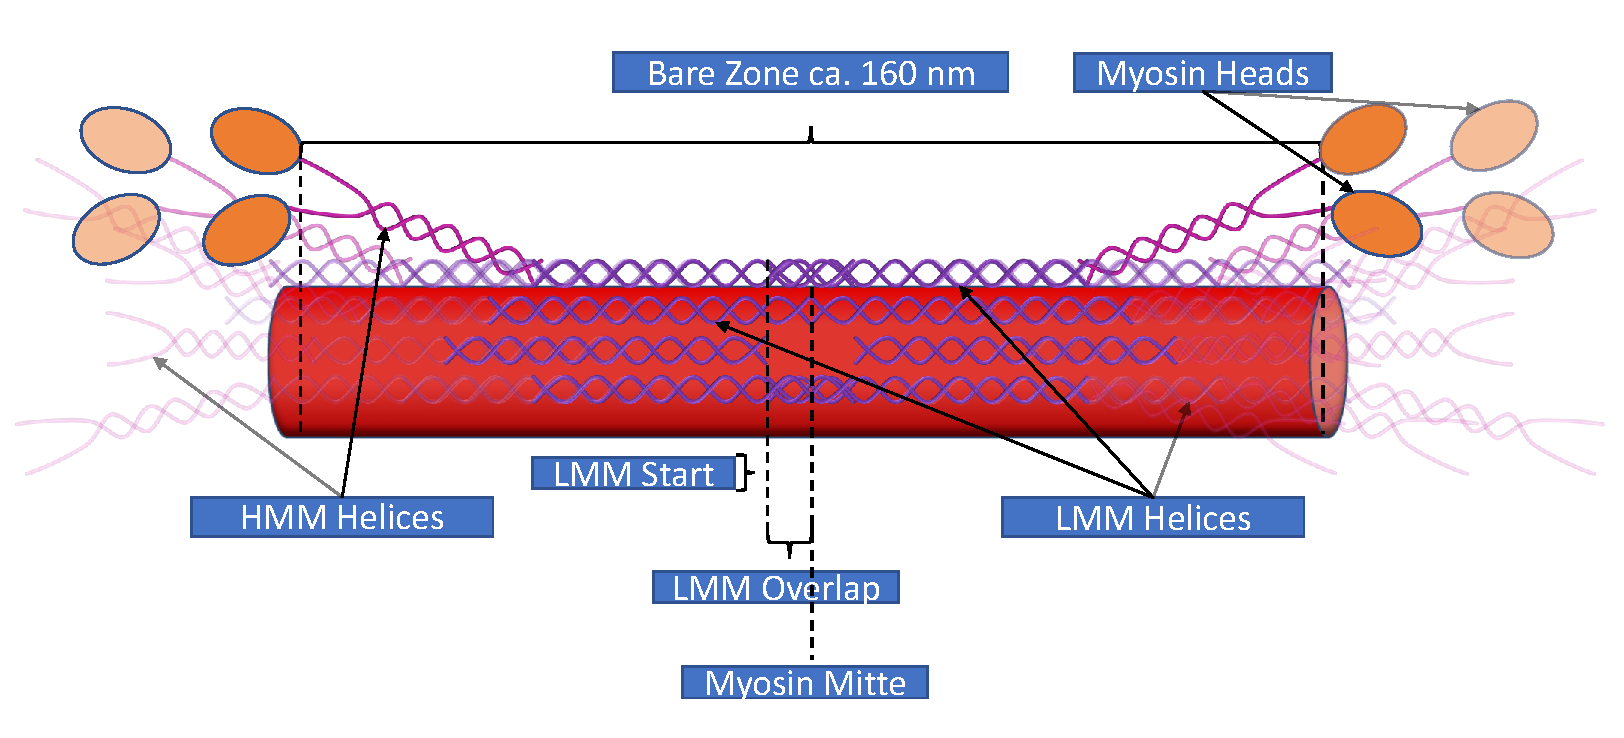
\includegraphics[width=1\textwidth]{Graphics/BareZone.pdf}
\caption{BareZone}
\label{fig:BareZone}
\end{figure}

\begin{figure}[h]
\center
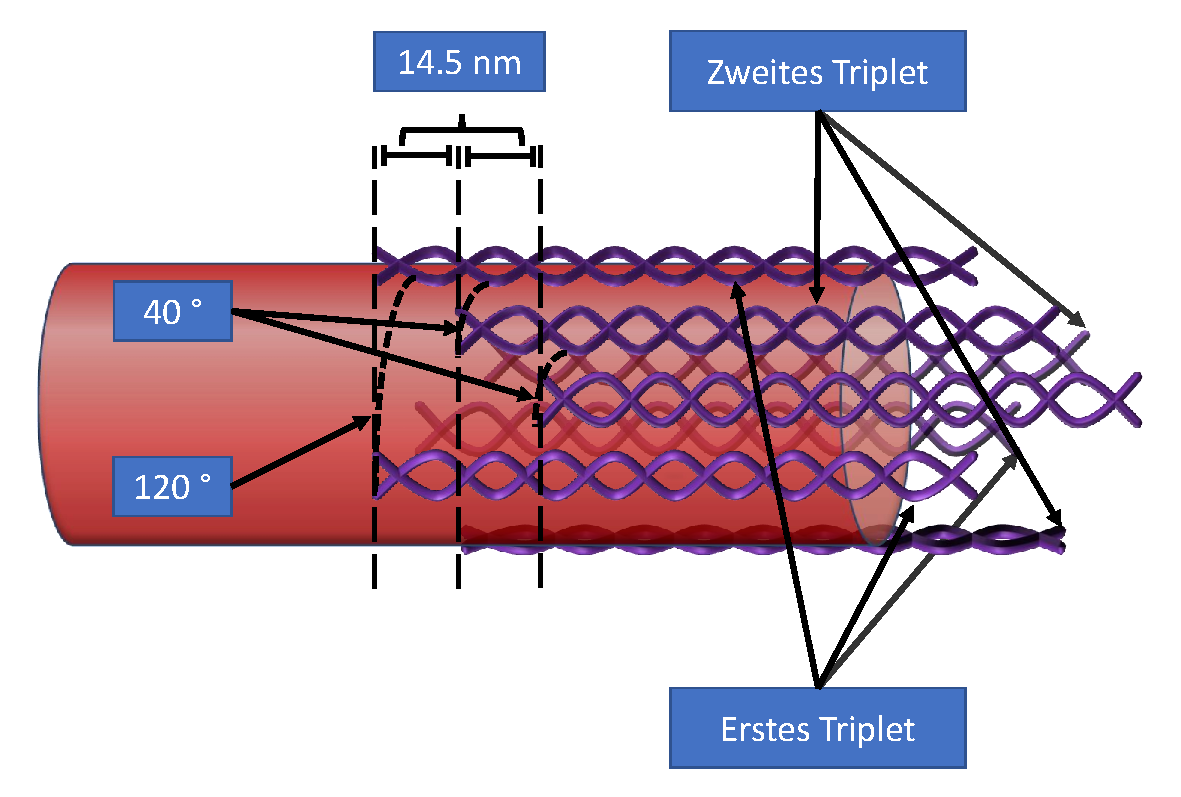
\includegraphics[width=1\textwidth]{Graphics/MeromyosinTriplets.pdf}
\caption{MeromyosinTriplets}
\label{fig:MeromyosinTriplets}
\end{figure}

Ein Myosin Filament lässt sich in diesem Modell grundlegend in drei Komponenten zerlegen. Einen zylinderförmigen Myosin Kern,
Doppelhelixförmiges Meromyosin und Eiförmige Myosinköpfe. Das Meromyosin wird weiterhin in einen HMM (heavy mero myosin) und einen LMM (light mero myosin) Teil aufgespalten.

Für den Myosinkern (ein drittel des Myosin radius) wird ein simpler Zylinder gerendert, da der Kern des Myosins für dieses Modell irrelevant ist.
Auf dem Myosinkern liegt in regelmäßigen Abständen ein Komplex aus LMM, HMM und Myosin köpfen. 
Dadurch, dass das Meromyosin von der Mitte des Myosins nach außen wächst gibt es in der Mitte einen relativ großen Bereich ohne Myosin köpfe. Dieser Bereich ist die sogenannte ``Barezone'' und entspricht ca. \(10\)\% der Länge des Myosins also rund \(160\)nm.

Die Anordnung der Meromyosin Komplexe ist wie folgt:
Drei Komplexe liegen auf gleicher Höhe auf dem Myosinkern in \(120\) Grad abständen nebeneinander. Dabei fängt die erste dieser  Dreierkonstellationen so an, dass die \textit{Barezone} \(160\) nm Länge hat. Dafür muss der erste Meromyosin Komplex schon vor der Mitte des Myosin Filaments anfangen.
In \(40\) nm Abständen wiederholt sich die Konstellation, wobei die drei Komplexe um \(40\) Grad rotiert werden (Reconditi:::). Der ganze Aufbau ist in  Abbildung \ref{fig:BareZone} und Abbildung \ref{fig:MeromyosinTriplets}

\paragraph{Berechnung der LMM Positionen}

\begin{figure}[!h]
\center
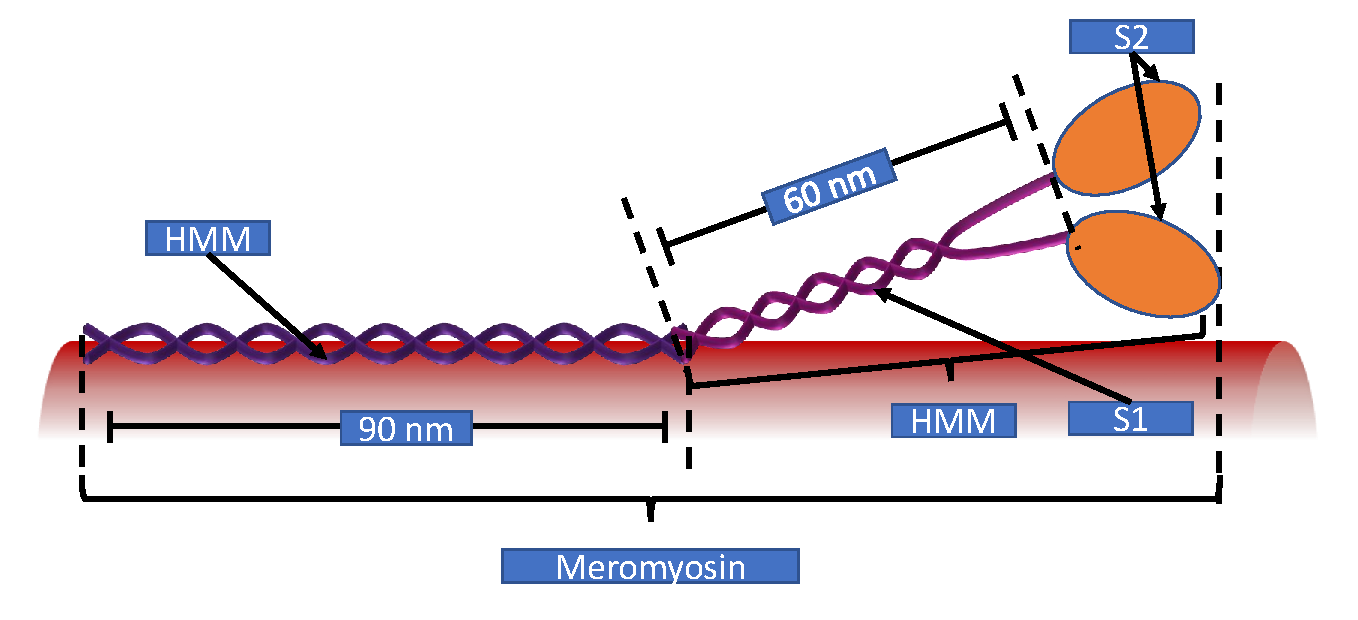
\includegraphics[width=1\textwidth]{Graphics/Meromyosin.pdf}
\caption{Meromyosin}
\label{fig:Meromyosin}
\end{figure}

Ein einzelnes LMM ist ca. \(90\) nm lang (Reconditi (::::)) und liegt direkt auf dem Myosin Kern (zu sehen in Abbildung \ref{fig:Meromyosin}). 
Jedes LMM wird durch eine Doppelhelix mit \(radiusHMM = radiusMyosinTrunk / 10\) repräsentiert. Für die erste Helix werden Stützpunkte berechnet anhand derer im Shader eine Linie generiert wird. Für die zweite Helix werden die Stützpunkte der ersten Helix dupliziert und um \(180\) Grad rotiert.
Die LMM Helices werden von der Mitte des Myosin Filaments nach außen hin Aufgebaut. Der Aufbau auf beiden Seiten ist Spiegel symmetrisch an der Mitte des Myosins, weswegen die Positionen nur für eine Hälfte generiert werden. Die Berechnung der Offset Positionen für die einzelnen LMM Teile ist in diesem Codebeispiel veranschaulicht(:::). Die Offset Positionen werden doppelt auf die Grafikkarte geladen und dort auf die entsprechende Myosin Hälfte transformiert.

\paragraph{Berechnung der HMM Positionen}

\begin{figure}[!h]
\center
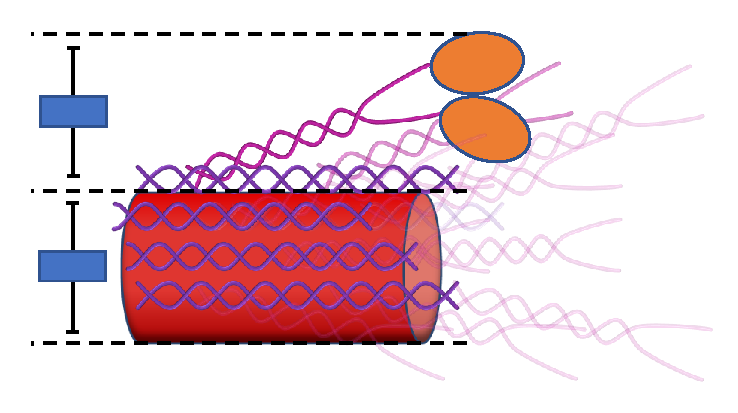
\includegraphics[width=1\textwidth]{Graphics/MyosinAufteilung.pdf}
\caption{MyosinAufteilung}
\label{fig:MyosinAufteilung}
\end{figure}

Das HMM gleicht von der Struktur her dem LMM und beginnt dort wo das LMM endet. Von dort aus spreizt es sich vom Myosin Kern ab (Abbildung \ref{fig:Meromyosin}). Der Winkel in dem das HMM Abgespreizt wird wird so gewählt, dass der Raum der von LMM und Myosin Kopf eingenommen wird zwei Drittel des Myosin entspricht(siehe Abbildung \ref{fig:MyosinAufteilung}).
Die Berechnung einer HMM Helix gleicht hauptsächlich der einer LMM Helix wobei die Helix nur \(60\) nm lang ist.
Am Ende der HMM helix ist ein kleiner Bereich an dem sich die beiden Helixstränge aufspalten und nicht mehr gewunden -, sonder gerade wachsen. Dabei wachsen die Stränge soweit auseinander, dass sich die Myosinköpfe die an ihnen hängen, die einen deutlich größeren Durchmesser als das HMM haben, nebeneinander Liegen ohne sich zu überschneiden.

\paragraph{Berechnung der Myosin Kopf positionen.}

Die Myosinköpfe werden in diesem Modell durch Ellipsoide repräsentiert.
Dabei ist die Lange Achse der Köpfe \(....\)nm und die kurze Achse  \(...\)nm lang.

Die Myosinköpfe befinden sich an jedem Ende einer HMM Helix, also befinden sich zwei Köpfe an einer HMM Doppelhelix.
Im Ruhezustand befindet sich die Lange Achse der Ellipsoide in einem \(....\) Grad Winkel zur HMM Helix. Dadurch wirken die Köpfe abgeknickt.

\subsection{Generierung von Aktin}
Alle Aktin Filamente haben die gleiche Geometrie bestehend aus einer Doppelhelix aus Aktin Monomeren durch welche sich Tropomyosin und Troponin flechten (siehe Abbildung \ref{fig:tropomyosinTroponin}). Deswegen bietet es sich wieder an, wie schon bei der Generierung von Myosin beschrieben, nur einmal die Geometrie für ein Aktin Filament zu erstellen und dann im Vertex Shader Instanzen dieser Geometrie an die passenden Offset Positionen zu verschieben.

\subsubsection{Generierung der Aktin Offset Positionen}
Im Gegensatz zur Myosin Generierung muss die Berechnung der Offset Positionen für die Aktin Filamente in vier verschiedene Fälle, einen für jeden Muskeltyp (siehe...), unterteilt werden.
Dies ist der Fall, da sich Sarkomere vor allem durch die strukturelle Anordnung der Aktin Filamente unterscheiden.
Bei allen betrachteten Sarkomer Typen ist dabei eine Sechseckige Anordnung der Aktin Filamente um jedes Myosin Filament zu beobachten. Allerdings unterscheiden sich die Sarkomer Typen durch den Grad der Besetzung dieses Sechseckigen Gitters um Jedes Myosin Filament.
Die Berechnung der offset Positionen für die jeweiligen Fälle läuft nun folgendermaßen ab: 
\paragraph{Fall 1 (Vertebrate simple und Vertebrate super \(2:1\))}

\begin{figure}[h]
\center
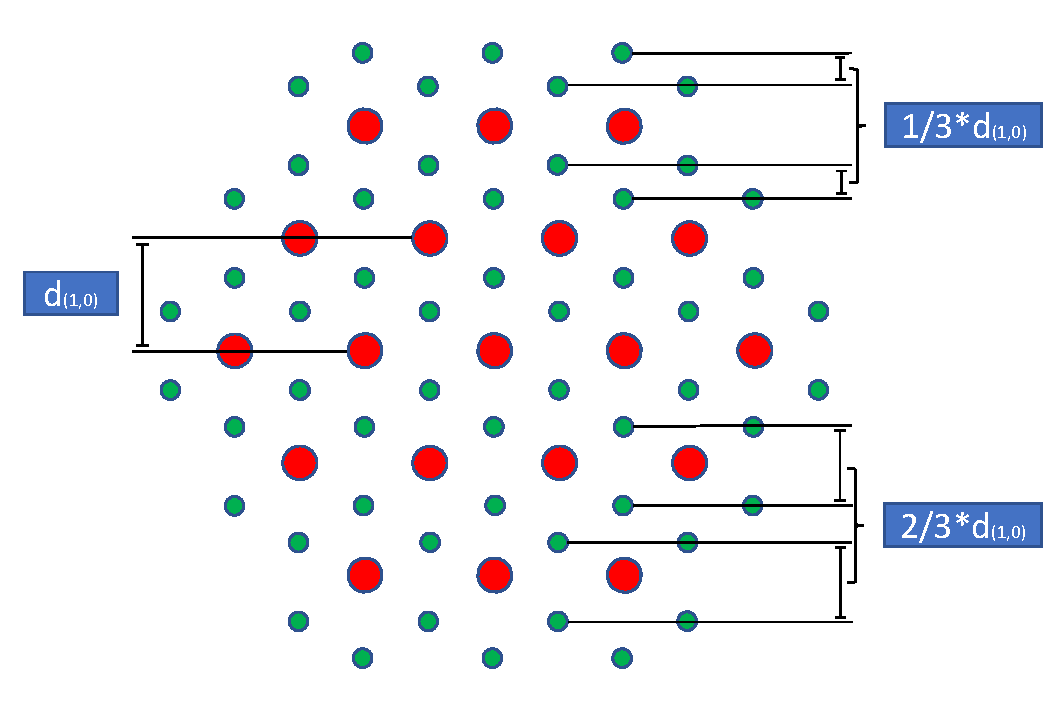
\includegraphics[width=0.8\textwidth]{Graphics/Actin2zu1Abstaende.pdf}
\caption{Aktin2zu1Abstände}
\label{fig:Aktin2zu1}
\end{figure}

Bei diesem Sarkomer Typ fallen auf jedes Myosin Filament zwei Aktin Filamente. Dabei sind um jeden Myosin Strang sechs Aktin Stränge Angeordnet wobei jedes Aktin Filament zum ``Aktin Ring''  von jeweils drei Myosin filamenten gehört. Das führt dann zu der in Abbildung \ref{fig:Aktin2zu1} gezeigten Struktur.
:::::::::::::::::::::::::::::::::::::::::::::::

\paragraph{Fall 2 (Insect Flight \(3:1\))}

\begin{figure}[h]
\center
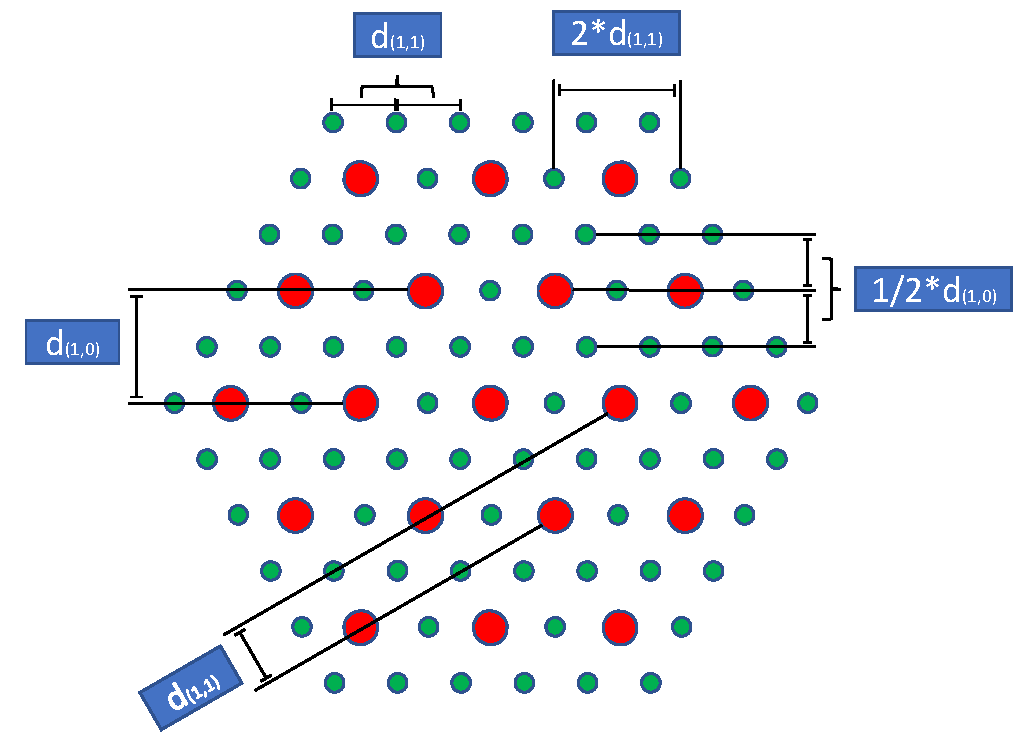
\includegraphics[width=0.8\textwidth]{Graphics/Actin3zu1Abstaende.pdf}
\caption{Aktin3zu1}
\label{fig:Aktin3zu1}
\end{figure}

In diesem Fall ist das Verhältnis zwischen Aktin und Myosin \(3:1\), was zu der in Abbildung \ref{fig:Aktin3zu1} dargestellten Strukturellen Anordnung der Aktin Filamente führt. In diesem Fall Wird ein Aktin Filament jeweils von zwei Myosin Filamenten geteilt.

Um die Positionsberechnung möglichst effizient zu gestalten, werden in diesem Fall die Offset Positionen Reihenweise Berechnet. 
Dadurch lässt sich wieder gewährleisten dass jede Position nur einmal Berechnet wird und am Ende keine suche nach doppelt berechneten Positionen nötig ist. Dabei ist vor allem der Symmetrische Aufbau des Sarkomers von Vorteil. Wenn man mit der Berechnung der Offset Positionen in der Mitte des Sarkomers beginnt, kann man pro Schleifendurchlauf immer die Hälfte einer Reihe mit Positionen Befüllen und diese Hälfte dann an der Mitte Spiegeln und anschließen die komplette Reihe Duplizieren und von der Mitte aus nach unten verschieben. Dadurch werden pro Schleifendurchlauf immer zwei Reihen, von der Mitte aus nach außen, mit Positionen Befüllt (siehe Abb.:::). Zwischen zwei Zeilen ist dabei jeweils ein Abstand von \(d11 = \frac{2 * d10}{\sqrt{3}}\). 
Die Berechnung der Offset Positionen pro Reihe unterteilt sich dabei in drei Fälle (siehe Abb....). 

Im ersten Fall werden in jeder zweiten Reihe mit einem Abstand von \(d11 = \frac{2 * d10}{\sqrt{3}}\) Aktin Positionen Erzeugt. Diese Position müssen Außerdem um \(0.5 * d11\) von der Mitte aus in \(x\) und \(-x\) Richtung verschoben werden.

Im zweiten und dritten Fall wird jeweils in der Lücke zwischen zwei Myosin Filamenten ein Aktin Filament platziert. Dadurch ergibt sich für diese Fälle ein Abstand von \(2 * d11\) zwischen zwei offset Positionen in einer Reihe. Der Unterschied zwischen beiden Fällen ist der initiale Offset in \(x\) und \(-x\) Richtung. 

Zum Schluss muss die Länge der Reihen, von der Mitte aus Abnehmend, passend begrenzt werden. Damit der Rand des Sarkomers von genau einer Schicht Aktin Filamente Beschränkt wird. 

Die Wahl des Richtigen Falls und der Passenden Reihenbeschränkung soll mit folgendem Codebeispiel veranschaulicht werden (...).

\paragraph{Fall 3 (Invertebrate \(5:1\))}

\begin{figure}[h]
\center
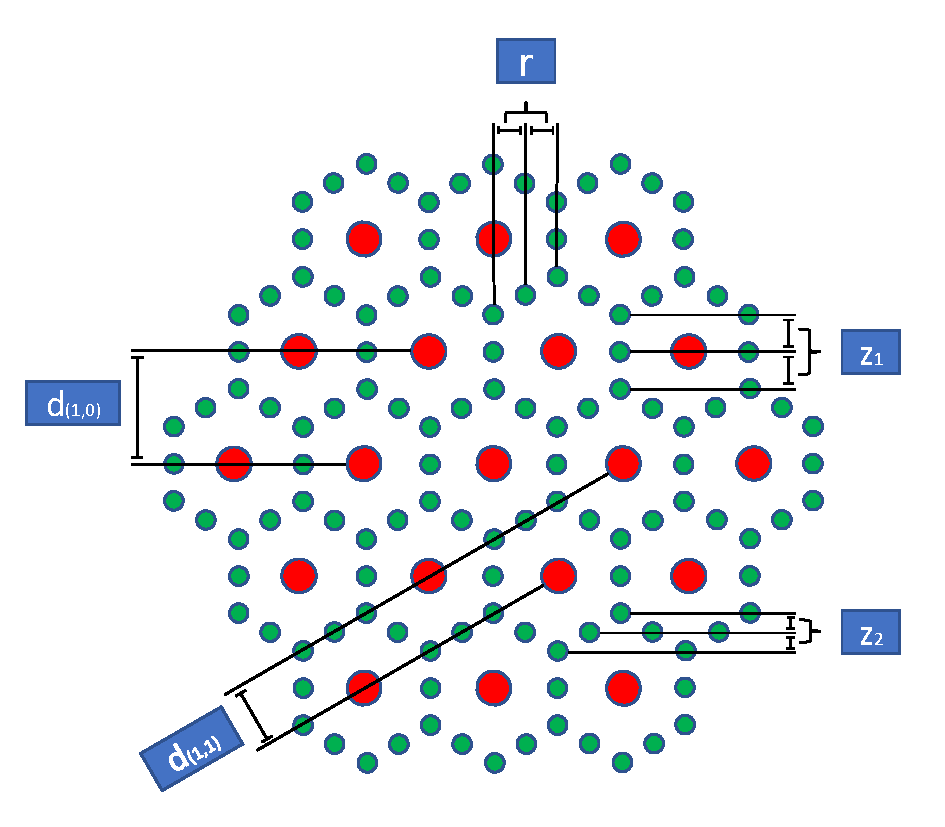
\includegraphics[width=0.8\textwidth]{Graphics/Actin5zu1Abstaende.pdf}
\caption{Aktin5zu1}
\label{fig:Aktin5zu1}
\end{figure}

Bei diesem Muskeltyp ist das Verhältnis zwischen Aktin und Myosin \(5:1\). Auch hier bietet es sich an die Offset Positionen für die Aktin Filamente Reihenweise von innen nach außen zu berechnen und sich dabei die Achsensymmetrie des Sarkomers zu nutze zu machen. Wie auch schon beim Aufbau für das (Insect Flight) Sarkomer werden in einer Schleife jeweils zwei Reihen pro Durchlauf generiert, wobei sich die Anordnung der Positionen pro Zeile wieder in drei Fälle aufteilen lässt (siehe Abbildung \ref{fig:Aktin5zu1}). Allerdings gibt bei diesem Sarkomer verschiedene Abstände zwischen den Zeilen. Dieser ist für a) \(zOffset =(\sqrt{3} / 3) * d11\) und für b) \(zOffset = d11 / 2\sqrt{3}\).

Der erste Fall für die Anordnung von Positionen in einer Reihe tritt alle vier Reihen auf. Dabei werden Positionen mit einem Abstand von \(d11\) zueinander und einem Initialen Offset von \(0.5 * d11\) gesetzt.

Der zweite und dritte Fall tritt immer für für jeweils drei aufeinander folgende reihen auf. Dabei alterniert die Anwendung der Erzeugungsregel des zweiten und dritten Falls und wird immer mit einer Reihe die Nach Fall eins erzeugt wurde begrenzt. 

Die Erzeugungsregel für den zweiten und dritten Fall Setzt in einer Reihe Aktin Positionen mit einem Abstand von \(2 * d11\).
Dabei gibt es beim zweiten Fall einen Initialen Offset von \(d11\).

Auch hier müssen die Reihen von der Mitte nach Außen abnehmend begrenzt werden um die Gewünschte Form des Sarkomers zu erhalten in der jedes Myosin Filament von jeweils zwölf Aktin Filamenten umschlossen wird.
Die Wahl des Richtigen Falls und der Passenden Reihenbeschränkung soll mit folgendem Codebeispiel veranschaulicht werden (...).

\paragraph{Fall 4 (Invertebrate \(6:1\))}

\begin{figure}[h]
\center
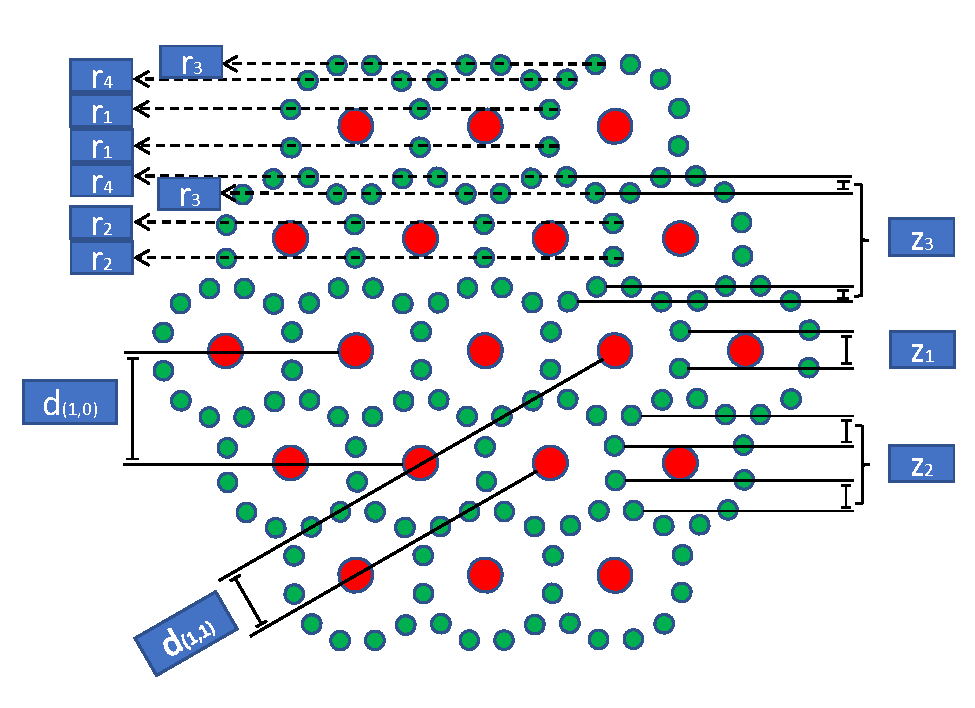
\includegraphics[width=0.8\textwidth]{Graphics/Actin6zu1Abstaende.pdf}
\caption{Aktin6zu1}
\label{fig:Aktin6zu1}
\end{figure}

Die Letzte Form eines Sarkomers das in dieser Arbeit behandelt wird gehört zu einem Invertebraten Muskel, bei dem auf ein Myosin Filament sechs Aktin Filamente anfallen. Wie in Abbildung \ref{fig:Aktin6zu1} zu sehen, erscheint die Anordnung der jeweils zwölf aktin Filamente um ein Myosin Filament ein Achteck zu sein. Allerdings lassen sich auch diese Filamente wieder auf einem Sechseckigen Gitter anordnen (siehe Abb...). Dabei würden die ecken des Sechsecks unbesetzt bleiben und auf jeder Kante zwei Aktin Filamente liegen. Diese Betrachtungsweise ermöglicht es unter anderem, die verschieden Sarkomertypen besser mit einander zu vergleichen.

Wie auch schon in den beiden vorherigen Fällen, erfolgt aus Effizienzgründen die Berechnung der Offset Positionen für die Aktin Filamente, reihenweise, von der Mitte nach Außen. Dabei unterteilt sich die reihenweise Erzeugung der Positionen in drei Fälle, wobei zwischen den Zeilen ein Abstand von 
\begin{equation}
a) Z_1 = (\sqrt{3} / 3) * d11
\end{equation}
\begin{equation}
b) Z_2 =((-6 + 5\sqrt{3}) / 6) * d11
\end{equation}
\begin{equation}
 oder c) Z_3 =(2 - \sqrt{3}) * d11
\end{equation}

Die erste und zweite Erzeugungsregel für Aktin Positionen in einer Reihe (\(r_1\) und \(r_2\)) wird immer für zwei aufeinander folgende Reihen angewandt. Dabei Alterniert die Anwendung der beiden Regeln. Auf diese Reihen folgen jeweils zwei Reihen die mit der dritten und vierten Erzeugungsregel befüllt werden. 
Die Positionen Innerhalb einer mit der ersten oder zweiten Erzeugungsregel generierten Reihe liegen jeweils \(2 * d11\) auseinander, wobei es im Ersten Fall noch einen Initialen Offset von \(d11\) in \(x\) und \(-x\) Richtung gibt.

Mit der dritten und vierten Erzeugungsregel (\(r_3\) und \(r_4\)) werden Reihen erzeugt bei denen der Abstand von Aktin Positionen innerhalb der Reihe alternierend entweder \((\sqrt{3} / 3) * d11\) oder \((2 - \sqrt{3} / 3) * d11\) ist. dabei sind immer zwei Aufeinander folgende Abstände gleich bevor sie wechseln. Bei Fall drei beginnt die Reihe in der Mitte mit dem Kurzen- und bei Fall vier mit dem langen Abstand. Jeweils zwei Aufeinanderfolgende Reihen die mit Erzeugungsregel drei oder vier erstellt wurden gehöhren zum selben Fall.

Auch hier müssen die Reihen von der Mitte nach Außen abnehmend begrenzt werden um die Gewünschte Form des Sarkomers zu erhalten in der jedes Myosin Filament von jeweils zwölf Aktin Filamenten umschlossen wird.
Die Wahl des Richtigen Falls und der Passenden Reihenbeschränkung soll mit folgendem Codebeispiel veranschaulicht werden (...).

\subsubsection{Generierung eines Aktin Filaments}

\begin{figure}[h]
\center
\includegraphics[width=1\textwidth]{Graphics/tropomyosinTroponin.pdf}
\caption{tropomyosinTroponin}
\label{fig:tropomyosinTroponin}
\end{figure}


Ein Aktin Filament setzt sich aus drei verschiedenen Komponenten zusammen. Aktin Monomere, Tropomyosin und Troponin. Den Hauptanteil haben dabei die Aktin Monomere, die sich in Form einer Doppelhelix Anordnen. Im Spalt zwischen den beiden Helices befindet sich Tropomyosin, welches am Anfang und am Ende jeweils von einem Troponin begrenzt wird. Ein Tropomyosin Abschnmitt umspannt dabei sieben Aktin Monomere. Der Aufbau wird in Abbildung  \ref{fig:tropomyosinTroponin} veranschaulicht.

\paragraph{Berechnung der Aktin Monomer Positionen}

\begin{figure}[h]
\center
\includegraphics[width=1\textwidth]{Graphics/AktinAufbau2.pdf}
\caption{AktinAufbau}
\label{fig:AktinAufbau}
\end{figure}

Ein Aktin Monomer wird in Diesem Modell als Kugel dargestellt. Um eine Helix zu erstellen, werden in einer For-Schleife vom Ursprung des Aktin Filaments aus, auf einander aufbauend Aktin Monomer Positionen berechnet. Damit sich die Monomere in der Doppelhelix berühren wird der Radius einses Aktion Monomers \(rMonomer\) halb so groß gewählt wie der Radius eines Aktin Filaments (rund...nm). Der Pitch der beiden Helices ist laut (...) \(37.5\) nm. Das entspricht in diesem Fall also einer halben Umdrehung einer einzelnen Helix. Der Aufbau wird in Abbildung \ref{fig:AktinAufbau} veranschaulicht.

Bei der Berechnung der Monomer Position wird wird das Aktin Monomer zunächst vom Mittelpunkt des Filaments um \(rMonomer\) nach außen verschoben. Danach wird das Monomer im Vergleich zu seinem Vorgänger um \(2*rMonomer\) das Filament entlang geschoben, und um \(helixPitch = 180 / (37.5 / 5.1????) = 28.32\) Grad um den Filamentmittelpunkt rotiert. Die zweite Helix der Doppelhelix wird  Gegenläufig zur Ersten generiert. Dazu reicht es aus das erste Aktin Monomer um \(180\) Grad im Vergleich zu seinem Gegenpart aus der anderen Helix zu rotieren.

Für Jedes Aktin Filament wird noch ein Gegenpaar Vorgemerkt, welches im Shader um \(180\) Grad rotiert, und dann auf die andere Seite des Sarkomers verschoben wird. Dadurch wird die gewünschte Form eines Sarkomers erreicht in der von beiden Enden Aktin Filamente in die Mitte des Sarkomers ``wachsen'' (siehe Abbildung \ref{fig:Sarkomer}).

\begin{figure}[h]
\center
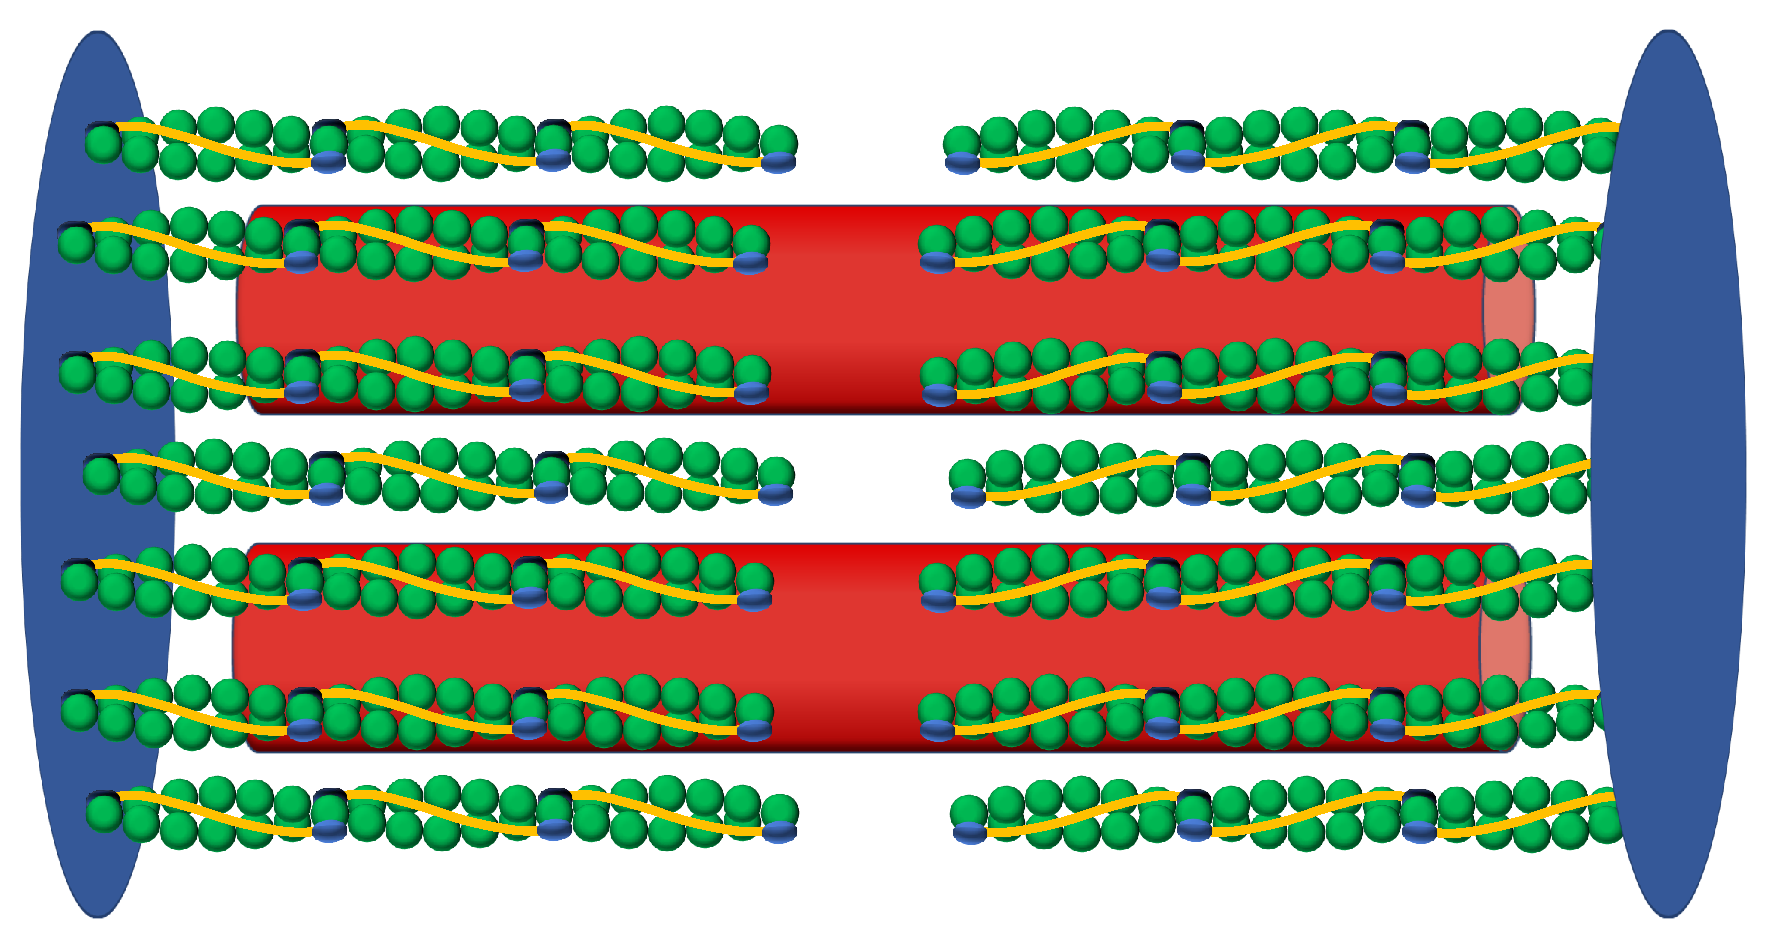
\includegraphics[width=1\textwidth]{Graphics/Sarkomer.pdf}
\caption{Sarkomer}
\label{fig:Sarkomer}
\end{figure}

\paragraph{Berechnung der Tropomyosin Positionen}

Ein Tropomyosin verläuft im Spalt zwischen der Aktin Doppelhelix und bindet dabei an sieben Aktin Monomere. Als Repräsentation für ein Tropomyosin wird eine gewundene Linie gerendert und so geshadet, dass ein dreidimensionaler Eindruck entsteht.

Vor dem Rendern müssen sowohl die Stützpunkte eines Linienzuges, als auch die Offset Positionen der einzelnen Linienzüge entlang der Doppelhelix berechnet werden. Die Stützpunkte eines Linienzuges werden Im gleichen Schleifendurchlauf wie die Aktin Monomere berechnet. Dabei wird auf Höhe der ersten sieben Monomer Positionen ein Tropomyosin Stützpunkt erstellt und in den Spalt zwischen die Doppelhelix verschoben.
Anschleßsend werden \(x = \left \lfloor{numMonomerPerActin / 7} \right \rfloor\) Offset Positionen und Rotationsmatrizen für die einzelnen Tropomyosin Proteine Berechnet. 

\paragraph{Berechnung der Troponin Positionen}

Die Enden eines Tropomyosins binden jeweils an ein Troponin (Reconditi...). Da jedes Tropomyosin an sieben Aktin Monomerere bindet, folgt daraus, dass auf Höhe jedes \(1,7,8,14,15,21,22,28...\) Aktin Monomers ein Troponin Platziert werden muss. Dies geschieht auch im Gleichen Schleifendurchlauf in dem die Aktin Monomere Platziert werden, da die grundlegende Rotration und Translation übernommen werden kann.

Jedes Troponin wird zunächst um \(rMonomer / 2\) nach außen geschoben um im Spalt zwischen den Aktin Helices zu liegen.
Danach wird es an die entsprechende Position im Spalt rotiert, wobei berücksichtigt werden muss, dass \(7 * helixPitch\) nicht genau \(180\) Grad entsprechen (siehe codebeispiel:...).

\subsection{Rendering}

Ein voll besetztes Modell eines Sarkomers besteht aus sehr viel Geometrie. In Hinsicht auf Übersichtlichkeit und Performanz wurde sich dafür entschieden alle Geometrie aus simplen Bausteinen zusammenzusetzen. Im Grunde besteht das Gesammte Modell aus drei Grundformen: Ellipsoide, Zylinder und Linenenzüge. Ein Invertebrate \(6:1\) Sarkomer mit \(547\) Myosin Filamenten und einer Länge von zwei Mikrometern besteht beispielsweise aus:
\begin{itemize}
\item  \(4.244.616\) Ellipsoiden (Aktin Monomere, Troponin und Myosin Köpfe)
\item  \(34.278.240\) Liniensegmenten (Tropomyosin, LMM und HMM)
\item \(547\) Zylindern (Myosin Kern).
\end{itemize}

Um diese Menge an Geometrie vernünftig Aussehen zu lassen und weiterhin eine Performance zu erreichen die es zulässt das Model Interaktiv zu benutzen, wurde beim Rendern auf diverse Kniffe zurückgegriffen.

\subsubsection{Rendern von Kugeln}
Wenn man Millionen von Kugeln Flüssig darstellen will, stößt ein Handelsüblicher Rechner sehr Schnell an seine Grenzen. Um dieses Problem zu lösen, wird eine Kugel nicht wie üblich durch Dreiecke angenähert, sondern mit geshadeten \textit{Pointsprites} dargestellt. Das beschleunigt den Rendering Prozess erheblich und hat, wenn man es richtig macht, visuell keine Einbußen.

In einem Renderaufruf werden also keine \textit{GL\_ TRIANGELS}, sondern \textit{GL\_ POINTS} gerendert. Diesen Punkten kann man im \textit{Fragment Shader} über \textit{gl\_ Pointsize} eine Größe geben. Diese Größe ist davon abhängig wie viele rasterisierte Pixel der Punkt im einnimmt. Daraus folgt, dass:
\begin{equation}
gl\_ PointSize = (basePointSize * viewport.y * focalLength.y) / gl\_ Position.w
\end{equation}
Dabei ist \(basePointSize\) z.B der Radius eines Aktin Monomers, \(viewport.y\) die y-Koordinate des verwendeten Viewports, \(focalLength.y\) die y-Komponente der Focal length der verwendeten Kamera und \(gl\_ Position.w\) die w-Komponente der Position des Punktes nach der Perspektivischen Transformation.

Im \textit{Fragment Shader} müssen mit 
\begin{equation}
length(gl\_ PointCoord * 2 - 1) <= 1
\end{equation}
zunächst die Pixel gefunden werden die innerhalb des darzustellenden Kreises liegen. \(gl\_ PointCoord\) ist dabei die 2D Position eines Fragments innerhalb eines \textit{GL\_ POINTS} der sich in x und y Richtung von \(-1\) bis \(1\) erstreckt . Das ist nötig, da mit \textit{GL\_ POINTS} üblicherweise kein Kreis, sondern ein Quadrat gerendert wird aus dem nun der Kreis geschnitten werden muss.

Für alle Fragmente die innerhalb des Kreises liegen muss nun eine Normale Berechnet werden. Die Normale wird dabei so gewählt, dass sie zu dem Punkt passt wenn er auf einer Kugeloberfläche liegen würde. (siehe (:::). Die Kugelnormale berechnet sich dabei wie folgt:
\begin{equation}
\begin{split}
sphereNormal.xy & = gl\_ PointCoord * vec2(2,-2) + vec2(-1, 1)\\
r & = dot(sphereNormal.xy, sphereNormal.xy)\\
sphereNormal.z & = \sqrt{1 - r}\\
sphereNormal & = normalize(sphereNormal).
\end{split}
\end{equation}

Zu diesem Zeitpunkt ist es möglich den Punkt mit normalem \textit{Phong Shading} so aussehen zu lassen wie eine Kugel. Allerdings haben diese Kugeln noch an jeder Position die selbe Tiefe was dazu führt, dass die kugeln beim bewegen der Szene immer übereinander Flippen. Um diesen unerwünschten Nebeneffekt zu beseitigen muss für jedes Fragment auf dem Kreis auch eine zur Kugel Passende Tiefe (\(gl\_ FragDepth\)) berechnet werden. Die Formel mit der sich die Passenden Tiefenwerte berechnen lassen ist die folgende:
\begin{equation}
gl\_ FragDepth = (clipSpacePos.z / clipSpacePos.w) * 0.5 + 0.5
\end{equation}
Dabei ist \(clipSpacePos.z\) und \(clipSpacePos.w\) die z- bzw. w-Komponente der Position des Fragments im Clip Space.
\subsubsection{Lines}

\subsection{Gui}

\section{Evaluation}

\section{Fazit}

\bibliographystyle{alphadin}
\bibliography{BA}
\end{document}